\documentclass{article}
\usepackage{parskip}
\usepackage{fullpage}
\usepackage{amsmath}
\usepackage{amssymb}
\usepackage{latexsym,paralist}
\usepackage{comment}
\usepackage{fancyvrb}
\usepackage{graphicx}
\usepackage{tikz}
\usetikzlibrary{arrows.meta}
\pagestyle{empty}

\includecomment{solution}
\excludecomment{solution}  % comment this out to create the solutions

\newcommand{\bs}{\noindent\textbf{Solution.}~}
\newcommand{\es}{\hfill $\square$}

\setcounter{secnumdepth}{-1}

\begin{document}
\subsection{IE 5545 A Network Game of Substitutes}
In a game of substitutes a player has a \emph{decreasing} incentive to choose an action as
more neighbors choose the action. Suppose that there are only two actions for each player,
0 or 1. In the ``Best-shot'' public goods game, a player will receive a benefit
of 1 if she or any of her neighbors take action 1. For example, if you or any of your
neighbors buy a drill you will benefit (assuming your neighbors will lend you the drill)
but there is a cost for purchasing the drill so you prefer that one of your neighbors
buys the drill. In this game the utility to player $i$ is
\begin{align*}
  u_i(1,S_{N_i}) &= 1 - c\\
  u_i(0,S_{N_i}) &= \begin{cases}
    1 \quad \text{if $a_j=1$ for some $j \in N_i$}\\
    0 \quad \text{if $a_j=0$ for all $j \in N_i$}
    \end{cases}
\end{align*}
where $N_i$ are the neighbors of player $i$, $S_{N_i}$ are the
strategies of the neighbors of player $i$, $a_j$ is the action taken
by player j, and $0 < c < 1$ is the cost for taking action 1.  Find a
pure strategy Nash equilibrium for the Best-shot public goods game
shown below that is different from the equilibrium given in class for
this game.

\vspace{.5in}
\begin{center}
\resizebox{.7\textwidth}{!}{%
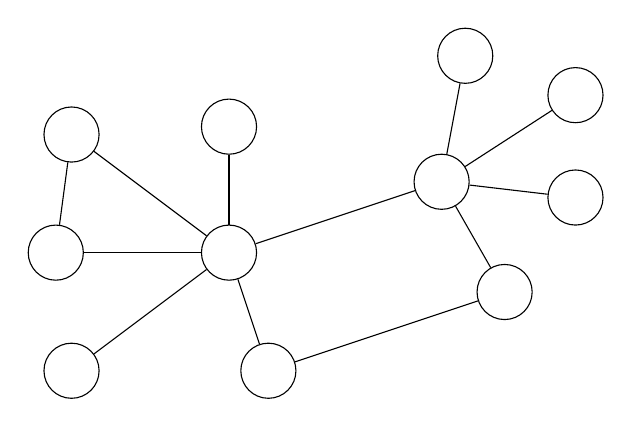
\begin{tikzpicture}
  \tikzstyle{every circle node}=[draw,inner sep=0pt,minimum size=7mm]
  
  \draw (0,0) node[circle] (A) {};
  \draw (2.7,.9) node[circle] (B) {};

  \draw (0,1.6) node[circle] (C) {};
  \draw (-2,1.5) node[circle] (D) {};
  \draw (-2.2,0) node[circle] (E) {};
  \draw (-2,-1.5) node[circle] (F) {};
 
  \draw (3,2.5) node[circle] (G) {};
  \draw (4.4,2) node[circle] (H) {};
  \draw (4.4,.7) node[circle] (I) {};
  \draw (3.5,-.5) node[circle] (J) {};
  \draw (.5,-1.5) node[circle] (K) {};

  \path (A) edge (B);
  \path (A) edge (C);
  \path (A) edge (D);
  \path (A) edge (E);
  \path (A) edge (F);
  \path (A) edge (K);

  \path (B) edge (G);
  \path (B) edge (H);
  \path (B) edge (I);
  \path (B) edge (J);

  \path (J) edge (K);
  \path (D) edge (E);

\end{tikzpicture}
}%
\end{center}

\end{document}
